\documentclass[border=1pt]{standalone}
\usepackage{tikz}
\usetikzlibrary{calc}
\usetikzlibrary{decorations.pathreplacing} % 使用扩号
\begin{document}
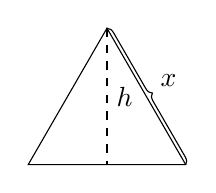
\begin{tikzpicture}
    % 绘制一个简单的三角形
    \coordinate (A) at (0,0);
    \coordinate (B) at (2,0);
    \coordinate (M) at (1,0);
    \coordinate (C) at (1,{sqrt(3)});

    \draw[decorate,decoration={brace,mirror}] (B) -- (C) node[midway,right=8pt,above=0.1pt] {$x$};
    % 绘制三角形
    \draw (A)  -- (B) -- (C) -- cycle;
    \draw[dashed] (C) -- (M) node[midway,right] {$h$} ;

\end{tikzpicture}
\end{document}


% convert -density 300 正三角形_带有高和边长注释.pdf 正三角形_带有高和边长注释.png